% Options for packages loaded elsewhere
\PassOptionsToPackage{unicode}{hyperref}
\PassOptionsToPackage{hyphens}{url}
\PassOptionsToPackage{dvipsnames,svgnames,x11names}{xcolor}
%
\documentclass[
]{article}
\usepackage{amsmath,amssymb}
\usepackage{lmodern}
\usepackage{iftex}
\ifPDFTeX
  \usepackage[T1]{fontenc}
  \usepackage[utf8]{inputenc}
  \usepackage{textcomp} % provide euro and other symbols
\else % if luatex or xetex
  \usepackage{unicode-math}
  \defaultfontfeatures{Scale=MatchLowercase}
  \defaultfontfeatures[\rmfamily]{Ligatures=TeX,Scale=1}
\fi
% Use upquote if available, for straight quotes in verbatim environments
\IfFileExists{upquote.sty}{\usepackage{upquote}}{}
\IfFileExists{microtype.sty}{% use microtype if available
  \usepackage[]{microtype}
  \UseMicrotypeSet[protrusion]{basicmath} % disable protrusion for tt fonts
}{}
\makeatletter
\@ifundefined{KOMAClassName}{% if non-KOMA class
  \IfFileExists{parskip.sty}{%
    \usepackage{parskip}
  }{% else
    \setlength{\parindent}{0pt}
    \setlength{\parskip}{6pt plus 2pt minus 1pt}}
}{% if KOMA class
  \KOMAoptions{parskip=half}}
\makeatother
\usepackage{xcolor}
\usepackage[margin=2cm]{geometry}
\usepackage{longtable,booktabs,array}
\usepackage{calc} % for calculating minipage widths
% Correct order of tables after \paragraph or \subparagraph
\usepackage{etoolbox}
\makeatletter
\patchcmd\longtable{\par}{\if@noskipsec\mbox{}\fi\par}{}{}
\makeatother
% Allow footnotes in longtable head/foot
\IfFileExists{footnotehyper.sty}{\usepackage{footnotehyper}}{\usepackage{footnote}}
\makesavenoteenv{longtable}
\usepackage{graphicx}
\makeatletter
\def\maxwidth{\ifdim\Gin@nat@width>\linewidth\linewidth\else\Gin@nat@width\fi}
\def\maxheight{\ifdim\Gin@nat@height>\textheight\textheight\else\Gin@nat@height\fi}
\makeatother
% Scale images if necessary, so that they will not overflow the page
% margins by default, and it is still possible to overwrite the defaults
% using explicit options in \includegraphics[width, height, ...]{}
\setkeys{Gin}{width=\maxwidth,height=\maxheight,keepaspectratio}
% Set default figure placement to htbp
\makeatletter
\def\fps@figure{htbp}
\makeatother
\setlength{\emergencystretch}{3em} % prevent overfull lines
\providecommand{\tightlist}{%
  \setlength{\itemsep}{0pt}\setlength{\parskip}{0pt}}
\setcounter{secnumdepth}{5}
\renewcommand{\arraystretch}{1.5}
\usepackage{tikz}
\usepackage{pgfplots}
\definecolor{nthu}{HTML}{7F1084}
\definecolor{secondary}{HTML}{910A17}
\definecolor{accent}{HTML}{410A91}
\ifLuaTeX
  \usepackage{selnolig}  % disable illegal ligatures
\fi
\IfFileExists{bookmark.sty}{\usepackage{bookmark}}{\usepackage{hyperref}}
\IfFileExists{xurl.sty}{\usepackage{xurl}}{} % add URL line breaks if available
\urlstyle{same} % disable monospaced font for URLs
\hypersetup{
  pdftitle={Deep-Learning-based DNA Sequence Fast Decoding},
  pdfauthor={Team NTHU-1},
  colorlinks=true,
  linkcolor={Maroon},
  filecolor={Maroon},
  citecolor={Blue},
  urlcolor={Blue},
  pdfcreator={LaTeX via pandoc}}

\title{Deep-Learning-based DNA Sequence Fast Decoding}
\author{Team NTHU-1}
\date{October 24, 2022}

\begin{document}
\maketitle

We read the
\href{https://www.ncbi.nlm.nih.gov/pmc/articles/PMC8015851/}{original
paper} mentioned in README of GitHub repository of this competition and
find the source code on
\href{https://github.com/GuanLab/Leopard}{GitHub}.

In this task, we would adopt this model, slightly modify it so that it's
suitable for newer \emph{Tensorflow} and tune its hyperparameters so as
to obtain the ideal performance.

\hypertarget{why-do-we-choose-this-model}{%
\section{Why do we choose this
model?}\label{why-do-we-choose-this-model}}

\hypertarget{more-accurate-more-efficiency}{%
\subsection{More accurate, more
efficiency}\label{more-accurate-more-efficiency}}

\begin{figure}
\centering
\includegraphics[width=0.87\textwidth,height=\textheight]{https://i.imgur.com/YmXiyKp.jpg}
\caption{Model performance, adapted from the original paper}
\end{figure}

As we can see in the picture, Leopard model outweighted \textbf{Anchor},
\textbf{FactorNet} and other state-of-the-art models in most of the
scenario.

Despite of its high accuracy, Leopard model also perform in stunning
speed, which no one can compete. That's the reason we adopt this model
as our target.

\hypertarget{model-structure}{%
\section{Model structure}\label{model-structure}}

This model, Leopard Unet, is composed of 4 main part: \textbf{Input},
\textbf{Encoder}, \textbf{Decoder} and \textbf{Output}.

\begin{figure}
\centering
\includegraphics[width=0.69\textwidth,height=\textheight]{https://i.imgur.com/ZNqZE65.png}
\caption{Diagram of the model, adapted from the original paper}
\end{figure}

\hypertarget{encoder}{%
\subsection{Encoder}\label{encoder}}

The \textbf{Encoder} comprises 5 \textbf{CCP}
\emph{(Convolution-Convolution-Pooling)} blocks, each of which contains
two 1D convolution layer and a max-pooling layer sequentially.

In each step, the length of data is divided by 5 during the process of
pooling.

\hypertarget{decoder}{%
\subsection{Decoder}\label{decoder}}

Similarly, 5 \textbf{UCC} \emph{(Upscaling-Convolution-Convolution)}
blocks constitute the \textbf{Decoder}. The upscaling component is
formed by 1D convolution-transpose layer. The first of the convolution
layer is concatenated to the second convolution layer in the
corresponding \textbf{CCP} block.

Each time, the length of data is 5 times as previous block due to
upscaling.

\hypertarget{details-of-model-layers}{%
\subsection{Details of Model Layers}\label{details-of-model-layers}}

There are 61 layers in total, all of which contain 475,969 parameters,
where 99.5\% or 474,017 ones are trainable.

\begin{longtable}[]{@{}
  >{\raggedright\arraybackslash}p{(\columnwidth - 6\tabcolsep) * \real{0.2570}}
  >{\centering\arraybackslash}p{(\columnwidth - 6\tabcolsep) * \real{0.2123}}
  >{\centering\arraybackslash}p{(\columnwidth - 6\tabcolsep) * \real{0.1173}}
  >{\raggedright\arraybackslash}p{(\columnwidth - 6\tabcolsep) * \real{0.4134}}@{}}
\caption{Layers of the model}\tabularnewline
\toprule()
\begin{minipage}[b]{\linewidth}\raggedright
Layer (type)
\end{minipage} & \begin{minipage}[b]{\linewidth}\centering
~~Output Shape~~
\end{minipage} & \begin{minipage}[b]{\linewidth}\centering
~Param \#~
\end{minipage} & \begin{minipage}[b]{\linewidth}\raggedright
Connected to
\end{minipage} \\
\midrule()
\endfirsthead
\toprule()
\begin{minipage}[b]{\linewidth}\raggedright
Layer (type)
\end{minipage} & \begin{minipage}[b]{\linewidth}\centering
~~Output Shape~~
\end{minipage} & \begin{minipage}[b]{\linewidth}\centering
~Param \#~
\end{minipage} & \begin{minipage}[b]{\linewidth}\raggedright
Connected to
\end{minipage} \\
\midrule()
\endhead
input\_1 (InputLayer) & (None, 10240, 5) & 0 & {[}{]} \\
conv1d (Conv1D) & (None, 10240, 15) & 540 &
{[}`input\_1{[}0{]}{[}0{]}'{]} \\
batch\_normalization (BatchNormalization) & (None, 10240, 15) & 60 &
{[}`conv1d{[}0{]}{[}0{]}'{]} \\
conv1d\_1 (Conv1D) & (None, 10240, 15) & 1590 &
{[}`batch\_normalization{[}0{]}{[}0{]}'{]} \\
batch\_normalization\_1 (BatchNormalization) & (None, 10240, 15) & 60 &
{[}`conv1d\_1{[}0{]}{[}0{]}'{]} \\
max\_pooling1d (MaxPooling1D) & (None, 5120, 15) & 0 &
{[}`batch\_normalization\_1{[}0{]}{[}0{]}'{]} \\
conv1d\_2 (Conv1D) & (None, 5120, 22) & 2332 &
{[}`max\_pooling1d{[}0{]}{[}0{]}'{]} \\
batch\_normalization\_2 (BatchNormalization) & (None, 5120, 22) & 88 &
{[}`conv1d\_2{[}0{]}{[}0{]}'{]} \\
conv1d\_3 (Conv1D) & (None, 5120, 22) & 3410 &
{[}`batch\_normalization\_2{[}0{]}{[}0{]}'{]} \\
batch\_normalization\_3 (BatchNormalization) & (None, 5120, 22) & 88 &
{[}`conv1d\_3{[}0{]}{[}0{]}'{]} \\
max\_pooling1d\_1 (MaxPooling1D) & (None, 2560, 22) & 0 &
{[}`batch\_normalization\_3{[}0{]}{[}0{]}'{]} \\
conv1d\_4 (Conv1D) & (None, 2560, 33) & 5115 &
{[}`max\_pooling1d\_1{[}0{]}{[}0{]}'{]} \\
batch\_normalization\_4 (BatchNormalization) & (None, 2560, 33) & 132 &
{[}`conv1d\_4{[}0{]}{[}0{]}'{]} \\
conv1d\_5 (Conv1D) & (None, 2560, 33) & 7656 &
{[}`batch\_normalization\_4{[}0{]}{[}0{]}'{]} \\
batch\_normalization\_5 (BatchNormalization) & (None, 2560, 33) & 132 &
{[}`conv1d\_5{[}0{]}{[}0{]}'{]} \\
max\_pooling1d\_2 (MaxPooling1D) & (None, 1280, 33) & 0 &
{[}`batch\_normalization\_5{[}0{]}{[}0{]}'{]} \\
conv1d\_6 (Conv1D) & (None, 1280, 49) & 11368 &
{[}`max\_pooling1d\_2{[}0{]}{[}0{]}'{]} \\
batch\_normalization\_6 (BatchNormalization) & (None, 1280, 49) & 196 &
{[}`conv1d\_6{[}0{]}{[}0{]}'{]} \\
conv1d\_7 (Conv1D) & (None, 1280, 49) & 16856 &
{[}`batch\_normalization\_6{[}0{]}{[}0{]}'{]} \\
batch\_normalization\_7 (BatchNormalization) & (None, 1280, 49) & 196 &
{[}`conv1d\_7{[}0{]}{[}0{]}'{]} \\
max\_pooling1d\_3 (MaxPooling1D) & (None, 640, 49) & 0 &
{[}`batch\_normalization\_7{[}0{]}{[}0{]}'{]} \\
conv1d\_8 (Conv1D) & (None, 640, 73) & 25112 &
{[}`max\_pooling1d\_3{[}0{]}{[}0{]}'{]} \\
batch\_normalization\_8 (BatchNormalization) & (None, 640, 73) & 292 &
{[}`conv1d\_8{[}0{]}{[}0{]}'{]} \\
conv1d\_9 (Conv1D) & (None, 640, 73) & 37376 &
{[}`batch\_normalization\_8{[}0{]}{[}0{]}'{]} \\
batch\_normalization\_9 (BatchNormalization) & (None, 640, 73) & 292 &
{[}`conv1d\_9{[}0{]}{[}0{]}'{]} \\
max\_pooling1d\_4 (MaxPooling1D) & (None, 320, 73) & 0 &
{[}`batch\_normalization\_9{[}0{]}{[}0{]}'{]} \\
conv1d\_10 (Conv1D) & (None, 320, 109) & 55808 &
{[}`max\_pooling1d\_4{[}0{]}{[}0{]}'{]} \\
batch\_normalization\_10 (BatchNormalization) & (None, 320, 109) & 436 &
{[}`conv1d\_10{[}0{]}{[}0{]}'{]} \\
conv1d\_11 (Conv1D) & (None, 320, 109) & 83276 &
{[}`batch\_normalization\_10{[}0{]}{[}0{]}'{]} \\
batch\_normalization\_11 (BatchNormalization) & (None, 320, 109) & 436 &
{[}`conv1d\_11{[}0{]}{[}0{]}'{]} \\
conv1d\_transpose (Conv1DTranspspose) & (None, 640, 72) & 15768 &
{[}`batch\_normalization\_11{[}0{]}{[}0{]}'{]} \\
concatenate (Concatenate) & (None, 640, 145) & 0 &
{[}`conv1d\_transpose{[}0{]}{[}0{]}',
`batch\_normalization\_9{[}0{]}{[}0{]}'{]} \\
conv1d\_12 (Conv1D) & (None, 640, 72) & 73152 &
{[}`concatenate{[}0{]}{[}0{]}'{]} \\
batch\_normalization\_12 (BatchNormalization) & (None, 640, 72) & 288 &
{[}`conv1d\_12{[}0{]}{[}0{]}'{]} \\
conv1d\_13 (Conv1D) & (None, 640, 72) & 36360 &
{[}`batch\_normalization\_12{[}0{]}{[}0{]}'{]} \\
batch\_normalization\_13 (BatchNormalization) & (None, 640, 72) & 288 &
{[}`conv1d\_13{[}0{]}{[}0{]}'{]} \\
conv1d\_transpose\_1 (Conv1DTranspose) & (None, 1280, 48) & 6960 &
{[}`batch\_normalization\_13{[}0{]}{[}0{]}'{]} \\
concatenate\_1 (Concatenate) & (None, 1280, 97) & 0 &
{[}`conv1d\_transpose\_1{[}0{]}{[}0{]}',
`batch\_normalization\_7{[}0{]}{[}0{]}'{]} \\
conv1d\_14 (Conv1D) & (None, 1280, 48) & 32640 &
{[}`concatenate\_1{[}0{]}{[}0{]}'{]} \\
batch\_normalization\_14 (BatchNormalization) & (None, 1280, 48) & 192 &
{[}`conv1d\_14{[}0{]}{[}0{]}'{]} \\
conv1d\_15 (Conv1D) & (None, 1280, 48) & 16176 &
{[}`batch\_normalization\_14{[}0{]}{[}0{]}'{]} \\
batch\_normalization\_15 (BatchNormalization) & (None, 1280, 48) & 192 &
{[}`conv1d\_15{[}0{]}{[}0{]}'{]} \\
conv1d\_transpose\_2 (Conv1DTranspose) & (None, 2560, 32) & 3104 &
{[}`batch\_normalization\_15{[}0{]}{[}0{]}'{]} \\
concatenate\_2 (Concatenate) & (None, 2560, 65) & 0 &
{[}`conv1d\_transpose\_2{[}0{]}{[}0{]}',
`batch\_normalization\_5{[}0{]}{[}0{]}'{]} \\
conv1d\_16 (Conv1D) & (None, 2560, 32) & 14592 &
{[}`concatenate\_2{[}0{]}{[}0{]}'{]} \\
batch\_normalization\_16 (BatchNormalization) & (None, 2560, 32) & 128 &
{[}`conv1d\_16{[}0{]}{[}0{]}'{]} \\
conv1d\_17 (Conv1D) & (None, 2560, 32) & 7200 &
{[}`batch\_normalization\_16{[}0{]}{[}0{]}'{]} \\
batch\_normalization\_17 (BatchNormalization) & (None, 2560, 32) & 128 &
{[}`conv1d\_17{[}0{]}{[}0{]}'{]} \\
conv1d\_transpose\_3 (Conv1DTranspose) & (None, 5120, 21) & 1365 &
{[}`batch\_normalization\_17{[}0{]}{[}0{]}'{]} \\
concatenate\_3 (Concatenate) & (None, 5120, 43) & 0 &
{[}`conv1d\_transpose\_3{[}0{]}{[}0{]}',
`batch\_normalization\_3{[}0{]}{[}0{]}'{]} \\
conv1d\_18 (Conv1D) & (None, 5120, 21) & 6342 &
{[}`concatenate\_3{[}0{]}{[}0{]}'{]} \\
batch\_normalization\_18 (BatchNormalization) & (None, 5120, 21) & 84 &
{[}`conv1d\_18{[}0{]}{[}0{]}'{]} \\
conv1d\_19 (Conv1D) & (None, 5120, 21) & 3108 &
{[}`batch\_normalization\_18{[}0{]}{[}0{]}'{]} \\
batch\_normalization\_19 (BatchNormalization) & (None, 5120, 21) & 84 &
{[}`conv1d\_19{[}0{]}{[}0{]}'{]} \\
conv1d\_transpose\_4 (Conv1DTranspose) & (None, 10240, 14) & 602 &
{[}`batch\_normalization\_19{[}0{]}{[}0{]}'{]} \\
concatenate\_4 (Concatenate) & (None, 10240, 29) & 0 &
{[}`conv1d\_transpose\_4{[}0{]}{[}0{]}',
`batch\_normalization\_1{[}0{]}{[}0{]}'{]} \\
conv1d\_20 (Conv1D) & (None, 10240, 14) & 2856 &
{[}`concatenate\_4{[}0{]}{[}0{]}'{]} \\
batch\_normalization\_20 (BatchNormalization) & (None, 10240, 14) & 56 &
{[}`conv1d\_20{[}0{]}{[}0{]}'{]} \\
conv1d\_21 (Conv1D) & (None, 10240, 14) & 1386 &
{[}`batch\_normalization\_20{[}0{]}{[}0{]}'{]} \\
batch\_normalization\_21 (BatchNormalization) & (None, 10240, 14) & 56 &
{[}`conv1d\_21{[}0{]}{[}0{]}'{]} \\
conv1d\_22 (Conv1D) & (None, 10240, 1) & 15 &
{[}`batch\_normalization\_21{[}0{]}{[}0{]}'{]} \\
\bottomrule()
\end{longtable}

\hypertarget{tuning}{%
\section{Tuning}\label{tuning}}

Below are the works that we tried to tune and optimize the performance
of the model.

\hypertarget{batch-size}{%
\subsection{Batch Size}\label{batch-size}}

In our experiments, we follow a hierarchical manner; that is, we first
tested \textbf{batch size}, then we adjusted \textbf{learning rate} for
a particular \textbf{batch size}.

\begin{figure}[htbp]
\centering
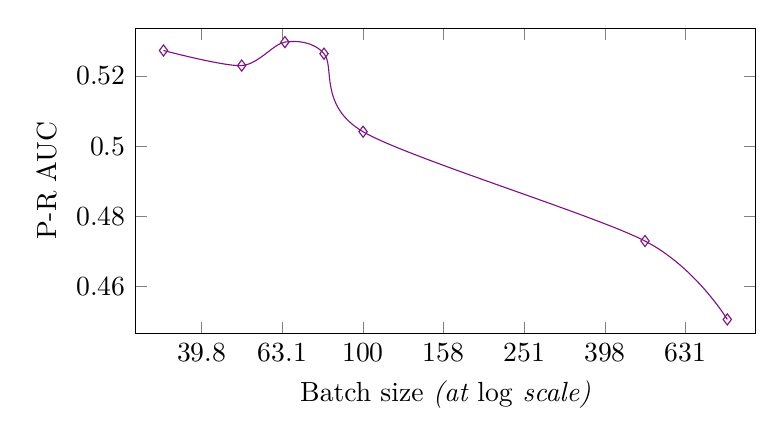
\begin{tikzpicture}
\begin{axis}[
    xlabel=Batch size \textit{(at $\log$ scale)},
    xmode=log,
    ylabel=P-R AUC,
    width=.78\linewidth,
    height=.45\linewidth,
    enlargelimits=0.05,
    legend pos=south east,
    log ticks with fixed point
]
\addplot[smooth, color=nthu, mark=diamond]
coordinates {
    (32, 0.5273)(50, 0.523)(64, 0.5297)(80, 0.5264)(100, 0.5041)(500, 0.4729)(800, 0.4505)
};
\end{axis}
\end{tikzpicture}
\caption{Maximum P-R AUC ever reached of various batch sizes}
\end{figure}

\hypertarget{section}{%
\subsubsection{32, 50}\label{section}}

We tried some smaller \textbf{batch size}s but their results were not so
good at all.

\hypertarget{section-1}{%
\subsubsection{64}\label{section-1}}

This is the best \textbf{batch size} we have ever found. We tested
several \textbf{learning rate}, such as \(0.001\), \(0.0025\),
\(0.005\), \(0.01\), \(0.025\), \(0.05\), among of which \(0.01\) gave
rise to optimal result.

\begin{figure}[htbp]
\centering
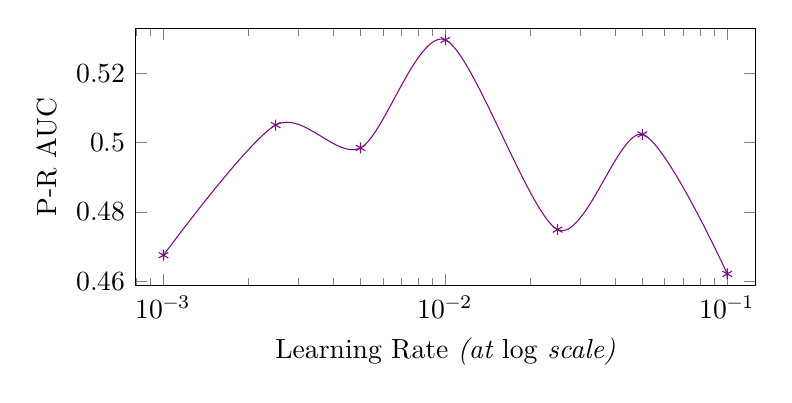
\begin{tikzpicture}
\begin{axis}[
    xlabel=Learning Rate \textit{(at $\log$ scale)},
    xmode=log,
    ylabel=P-R AUC,
    width=.78\linewidth,
    height=.4\linewidth,
    enlargelimits=0.05,
    legend pos=south east
]
\addplot[smooth, color=nthu, mark=asterisk]
coordinates {
    (0.001, 0.4675)(0.0025, 0.5051)(0.005, 0.4985)(0.01, 0.5297)(0.025, 0.4749)(0.05, 0.5024)(0.1, 0.4621)
};
\end{axis}
\end{tikzpicture}
\caption{Maximum P-R AUC of several learning rates}
\end{figure}

\hypertarget{section-2}{%
\subsubsection{100}\label{section-2}}

This is the default value. The maximum of \emph{P-R AUC
(Precision-Recall Area Under Curve)} could be up to \(0.5\), which was
better than the baseline CNN model.

\hypertarget{section-3}{%
\subsubsection{500}\label{section-3}}

We encounter severe \emph{\textbf{overfitting}} when it comes to this
\textbf{batch size}; that is, \emph{P-R AUC} could increase up to about
\(0.96\) for the training set, whereas the ones for validation set were
as low as \(0.25\). What's worse, since we increased the patience of
early stop to 10, it exhausted the 2-hour wall time.

\begin{figure}[htbp]
\centering
\begin{tikzpicture}
\begin{axis}[
    xlabel=Epoch,
    ylabel=P-R AUC,
    width=.78\linewidth,
    height=.4\linewidth,
    enlargelimits=0.05,
    legend pos=south east
]
\addplot[smooth, secondary] table [col sep=comma] {train.csv};
\addplot[smooth, accent] table [col sep=comma] {valid.csv};
\legend{Training, Validation}
\end{axis}
\end{tikzpicture}
\caption{P-R AUC changes during epoches: Training vs. Validation data set}
\end{figure}

\hypertarget{section-4}{%
\subsubsection{800}\label{section-4}}

The maximum \textbf{batch size} for V100 is 800 since it consumes about
31GB GPU memory. For this \textbf{batch size}, the coverage rate of
validation loss were quite slow despite of \textbf{learning rate}. As a
consequence, the results were also not so good.

\begin{figure}[htbp]
\centering
\begin{tikzpicture}
\begin{axis}[
    xlabel=Epoch,
    ylabel=Validation Loss \textit{(at $\log$ scale)},
    ymode=log,
    width=.78\linewidth,
    height=.5\linewidth,
    enlargelimits=0.05,
    legend pos=north east
]
\addplot[smooth, accent] table [col sep=comma] {loss_800.csv};
\addplot[smooth, nthu] table [col sep=comma] {loss_100.csv};
\addplot[smooth, secondary] table [col sep=comma] {loss_64.csv};
\legend{Batch size 800, Batch size 100, Batch size 64}
\end{axis}
\end{tikzpicture}
\caption{Loss convergence (Note that the curve of batch size 800 never under $10^{-3}$)}
\end{figure}

\hypertarget{section-5}{%
\subsubsection{1600, 2000, 2500}\label{section-5}}

These three \textbf{batch size}s were only measured on A100 for sure.
Their results were quite similar to 800.

\hypertarget{parallelization-via-multiple-gpus}{%
\subsection{Parallelization via Multiple
GPUs}\label{parallelization-via-multiple-gpus}}

We also managed to parallelize the training and utilized multiple GPUs.
Nonetheless, the performance would decline a lot. Furthermore, the
metrics would drop suddenly and dramatically after the number of GPU was
over a value. We guessed that it might due to the simple, linear scale
of \textbf{learning rate}, trying to find ad-hoc optimal
\textbf{learning rate} for different number of GPU yet in vain.

Eventually, we decide to train on only a single GPU since we believe
that the performance counts more. Still, we provide the job script to
train across two A100s.

\begin{figure}[htbp]
\centering
\begin{tikzpicture}
\begin{axis}[
    xlabel=\# GPU,
    xmin=0.5, xmax=4.5,
    xtick distance=1,
    ylabel=P-R AUC,
    width=.78\linewidth,
    height=.5\linewidth,
    enlargelimits=0.05,
    legend pos=south east
]
\addplot[smooth, color=nthu, mark=Mercedes star]
coordinates {
    (1, 0.5297)(2, 0.4815)(3, 0.4461)(4, 0.4780)
};
\end{axis}
\end{tikzpicture}
\caption{Maximum P-R AUC of \# GPU}
\end{figure}

\hypertarget{volta-and-ampuxe8re-gpus}{%
\subsection{Volta and Ampère GPUs}\label{volta-and-ampuxe8re-gpus}}

The main GPUs of Gadi are NVIDIA Volta V100 cards. Nevertheless, there
are 2 DGX-A100 node on Gadi equipped with the newest on the market so
far NVIDIA Ampère A100 cards.

It's no doubt that the process of training becomes faster since A100 is
more powerful than V100.

In addition, A100 is of 80GB memory, whereas there is only 32GB on V100.
As a consequence, \textbf{batch size} could be far more larger.

\pagebreak

\hypertarget{result}{%
\section{Result}\label{result}}

The best performance of the metrics we have ever achieved were under
following condition:

\begin{description}
\tightlist
\item[Batch Size]
64
\item[Learning Rate]
0.01
\item[\# GPU]
1
\end{description}

\begin{longtable}[]{@{}
  >{\centering\arraybackslash}p{(\columnwidth - 10\tabcolsep) * \real{0.0775}}
  >{\centering\arraybackslash}p{(\columnwidth - 10\tabcolsep) * \real{0.2326}}
  >{\centering\arraybackslash}p{(\columnwidth - 10\tabcolsep) * \real{0.1628}}
  >{\centering\arraybackslash}p{(\columnwidth - 10\tabcolsep) * \real{0.1395}}
  >{\centering\arraybackslash}p{(\columnwidth - 10\tabcolsep) * \real{0.2326}}
  >{\raggedleft\arraybackslash}p{(\columnwidth - 10\tabcolsep) * \real{0.1550}}@{}}
\caption{Performance of Single GPU}\tabularnewline
\toprule()
\begin{minipage}[b]{\linewidth}\centering
GPU Type
\end{minipage} & \begin{minipage}[b]{\linewidth}\centering
Loss \emph{(Binary Crossentropy)}
\end{minipage} & \begin{minipage}[b]{\linewidth}\centering
~P-R AUC~
\end{minipage} & \begin{minipage}[b]{\linewidth}\centering
Dice coefficient
\end{minipage} & \begin{minipage}[b]{\linewidth}\centering
Binary Intersection of Union
\end{minipage} & \begin{minipage}[b]{\linewidth}\raggedleft
Training Time {[}s{]}
\end{minipage} \\
\midrule()
\endfirsthead
\toprule()
\begin{minipage}[b]{\linewidth}\centering
GPU Type
\end{minipage} & \begin{minipage}[b]{\linewidth}\centering
Loss \emph{(Binary Crossentropy)}
\end{minipage} & \begin{minipage}[b]{\linewidth}\centering
~P-R AUC~
\end{minipage} & \begin{minipage}[b]{\linewidth}\centering
Dice coefficient
\end{minipage} & \begin{minipage}[b]{\linewidth}\centering
Binary Intersection of Union
\end{minipage} & \begin{minipage}[b]{\linewidth}\raggedleft
Training Time {[}s{]}
\end{minipage} \\
\midrule()
\endhead
V100 & \(7.2768\times10^{-4}\) & \(0.5297\) & \(0.3705\) & \(0.3625\) &
\(3170.19\) \\
A100 & \(7.3153\times10^{-4}\) & \(0.5288\) & \(0.4109\) & \(0.3701\) &
\(941.63\) \\
\bottomrule()
\end{longtable}

Just as the above table shown, the training time of A100 was
approximately a third of the one of V100 whereas other metrics were of
little difference.

\end{document}
